% Options for packages loaded elsewhere
\PassOptionsToPackage{unicode}{hyperref}
\PassOptionsToPackage{hyphens}{url}
%
\documentclass[
  12pt,
  a4paper]{extarticle}
\title{Further Examples --- Limits Inferior and Superior}
\author{Christian Jones: University of Bath}
\date{November 2022}

\usepackage{amsmath,amssymb}
\usepackage{lmodern}
\usepackage{iftex}
\ifPDFTeX
  \usepackage[T1]{fontenc}
  \usepackage[utf8]{inputenc}
  \usepackage{textcomp} % provide euro and other symbols
\else % if luatex or xetex
  \usepackage{unicode-math}
  \defaultfontfeatures{Scale=MatchLowercase}
  \defaultfontfeatures[\rmfamily]{Ligatures=TeX,Scale=1}
\fi
% Use upquote if available, for straight quotes in verbatim environments
\IfFileExists{upquote.sty}{\usepackage{upquote}}{}
\IfFileExists{microtype.sty}{% use microtype if available
  \usepackage[]{microtype}
  \UseMicrotypeSet[protrusion]{basicmath} % disable protrusion for tt fonts
}{}
\makeatletter
\@ifundefined{KOMAClassName}{% if non-KOMA class
  \IfFileExists{parskip.sty}{%
    \usepackage{parskip}
  }{% else
    \setlength{\parindent}{0pt}
    \setlength{\parskip}{6pt plus 2pt minus 1pt}}
}{% if KOMA class
  \KOMAoptions{parskip=half}}
\makeatother
\usepackage{xcolor}
\IfFileExists{xurl.sty}{\usepackage{xurl}}{} % add URL line breaks if available
\IfFileExists{bookmark.sty}{\usepackage{bookmark}}{\usepackage{hyperref}}
\hypersetup{
  pdftitle={Further Examples --- Limits Inferior and Superior},
  pdfauthor={Christian Jones: University of Bath},
  hidelinks,
  pdfcreator={LaTeX via pandoc}}
\urlstyle{same} % disable monospaced font for URLs
\usepackage[margin=2.5cm]{geometry}
\usepackage{longtable,booktabs,array}
\usepackage{calc} % for calculating minipage widths
% Correct order of tables after \paragraph or \subparagraph
\usepackage{etoolbox}
\makeatletter
\patchcmd\longtable{\par}{\if@noskipsec\mbox{}\fi\par}{}{}
\makeatother
% Allow footnotes in longtable head/foot
\IfFileExists{footnotehyper.sty}{\usepackage{footnotehyper}}{\usepackage{footnote}}
\makesavenoteenv{longtable}
\usepackage{graphicx}
\makeatletter
\def\maxwidth{\ifdim\Gin@nat@width>\linewidth\linewidth\else\Gin@nat@width\fi}
\def\maxheight{\ifdim\Gin@nat@height>\textheight\textheight\else\Gin@nat@height\fi}
\makeatother
% Scale images if necessary, so that they will not overflow the page
% margins by default, and it is still possible to overwrite the defaults
% using explicit options in \includegraphics[width, height, ...]{}
\setkeys{Gin}{width=\maxwidth,height=\maxheight,keepaspectratio}
% Set default figure placement to htbp
\makeatletter
\def\fps@figure{htbp}
\makeatother
\setlength{\emergencystretch}{3em} % prevent overfull lines
\providecommand{\tightlist}{%
  \setlength{\itemsep}{0pt}\setlength{\parskip}{0pt}}
\setcounter{secnumdepth}{5}
\newcommand{\BOO}{BOO}
\usepackage{float}
\ifLuaTeX
  \usepackage{selnolig}  % disable illegal ligatures
\fi

\usepackage{amsthm}
\theoremstyle{plain}
\newtheorem*{theorem*}{Theorem}\newtheorem{theorem}{Theorem}[section]
\theoremstyle{plain}
\newtheorem*{lemma*}{Lemma}\newtheorem{lemma}{Lemma}[section]
\theoremstyle{plain}
\newtheorem*{corollary*}{Corollary}\newtheorem{corollary}{Corollary}[section]
\theoremstyle{plain}
\newtheorem*{proposition*}{Proposition}\newtheorem{proposition}{Proposition}[section]
\theoremstyle{plain}
\newtheorem*{conjecture*}{Conjecture}\newtheorem{conjecture}{Conjecture}[section]
\theoremstyle{definition}
\newtheorem*{definition*}{Definition}\newtheorem{definition}{Definition}[section]
\theoremstyle{definition}
\newtheorem*{example*}{Example}\newtheorem{example}{Example}[section]
\theoremstyle{definition}
\newtheorem*{exercise*}{Exercise}\newtheorem{exercise}{Exercise}[section]
\theoremstyle{remark}
\newtheorem*{remark*}{Remark}
\newtheorem*{solution*}{Solution}
\let\BeginKnitrBlock\begin \let\EndKnitrBlock\end


%\usepackage[english,shorthands=off]{babel}
\usepackage{etoolbox}
\usepackage{spverbatim}
\makeatletter
\@ifpackageloaded{float}{}{\usepackage{float}}
\@ifpackageloaded{adjustbox}{}{\usepackage[Export]{adjustbox}}
\makeatother
\floatplacement{figure}{H}
\newcommand{\scalefactor}{1.2}
\adjustboxset*{min width=\scalefactor\width,max width=\linewidth}
\renewcommand{\familydefault}{phv}
\fontfamily{phv}\selectfont
\renewcommand{\em}{\bf}\renewcommand{\textit}{\textbf}\renewcommand{\emph}{\textbf}\renewcommand{\it}{\bf}\renewcommand{\itshape}{\bf}
\setlength{\parindent}{0.0pt}
\setlength{\parskip}{1.0\baselineskip}
\renewcommand{\baselinestretch}{1.5}\selectfont
\setlength{\mathsurround}{0.2em}
\setlength{\arraycolsep}{0.5cm}\renewcommand{\arraystretch}{1.5}
\addtolength{\jot}{\baselineskip}
\renewcommand{\;}{\,}
\sloppy
\allowdisplaybreaks
\usepackage{amsthm}
\newtheoremstyle{plain}{20pt}{3pt}{}{}{\bfseries}{.\newline\nobreak}{1.0em\nobreak}{}
\newtheoremstyle{definition}{20pt}{3pt}{}{}{\bfseries}{.\newline\nobreak}{1.0em\nobreak}{}
\newtheoremstyle{remark}{20pt}{3pt}{}{}{\bfseries}{.\newline\nobreak}{1.0em\nobreak}{}
\csundef{Proof}
\csundef{endProof}
\newenvironment{Proof}
  {\noindent{\bf Proof.}\hspace*{1em}}% Begin
  {\qed\par}% End
%% When redefining an environment it is vital that it has 
%% the same number of arguments as the original
\renewenvironment{proof}[1][\proofname]
  {\trivlist\item\relax\noindent{\bf {#1}.}\hspace*{1em}}% Begin
  {\qed\endtrivlist}% End

\begin{document}
\maketitle

{
\setcounter{tocdepth}{2}
\tableofcontents
}
\newpage
\pagenumbering{arabic}

\hypertarget{overview}{%
\section*{Overview}\label{overview}}
\addcontentsline{toc}{section}{Overview}

In this document, you'll find three different examples of finding the limit superior (\(\limsup\)) and limit inferior (\(\liminf\)) of a sequence, with different methods used in each case.

\hypertarget{example-1}{%
\subsection*{Example 1}\label{example-1}}
\addcontentsline{toc}{subsection}{Example 1}

\BeginKnitrBlock{example}
{\label{exm:ex1} }Consider the sequence \((a_n)_{n}\) defined by \[a_n = (-1)^n\frac{2n}{1+3n}.\] Find \(\limsup_{n \to \infty} a_n\) and \(\liminf_{n \to \infty} a_n\).
\EndKnitrBlock{example}

\textbf{Solution}
Firstly, note that we can rewrite each \(a_n\) as \[a_n = (-1)^n \frac{2}{3}\frac{1}{\frac{1}{3n} + 1}.\] Splitting into odd and even cases, we obtain \[a_n = \begin{cases} \frac{2}{3}\frac{1}{\frac{1}{3n} + 1} &\quad \text{for $n$ even},\\
\frac{2}{3}\frac{-1}{\frac{1}{3n} + 1} &\quad \text{for $n$ odd}.\end{cases}\] Note that for \(j \in \mathbb{N}\), \(a_{2j-1} \leq 0 \leq a_{2j}\). Also note that \((a_{2j-1})_j\) is a decreasing sequence and \((a_{2j})_{j}\) is an increasing sequence {[}Try showing these!{]} Moreover, \(\lvert a_n \rvert \leq \frac{2}{3} \; \forall n\in\mathbb{N}\), so \((a_n)_n\) is bounded.

Now, fix \(k \in \mathbb{N}\). We have:
\begin{align*}
\sup_{k\geq n}a_n &= \sup_{2j \geq k} a_{2j}, \; \; &&\text{(since only even elements are non-negative.)}\\
&= \lim_{j \to \infty} a_{2j}, \; \; &&\text{(since $(a_{2j})_j$ is a bounded increasing sequence)},\\
&= \frac{2}{3}. \; \; \quad &&\text{(by algebra of limits)}
\end{align*}
Hence, taking \(k \to \infty\), we find that \(\sup_{n \geq k} a_n \to \frac{2}{3}\). So, \(\limsup_{n \to \infty} a_n = \frac{2}{3}\).

Similarly, fixing \(k \in \mathbb{N}\) again:
\begin{align*}
\inf_{k\geq n}a_n &= \inf_{2j \geq k} a_{2j-1}, \; \; &&\text{(since only odd elements are non-positive.)}\\
&= \lim_{j \to \infty} a_{2j-1}, \; \; &&\text{(since $(a_{2j-1})_j$ is a bounded decreasing sequence)},\\
&= \lim_{j \to \infty}-\frac{4-\frac{2}{j}}{6 - \frac{2}{j}}, \; \; \quad &&\text{(by sequence definition)}\\
&= -\frac{2}{3}. \; \; \quad &&\text{(by algebra of limits)}.
\end{align*}

Hence, taking \(k \to \infty\), we find that \(\inf_{n \geq k} a_n \to -\frac{2}{3}\). So, \(\liminf_{n \to \infty} a_n = -\frac{2}{3}\).

In case you're interested, the first 100 terms of the sequence \((a_n)_n\) looks like this:

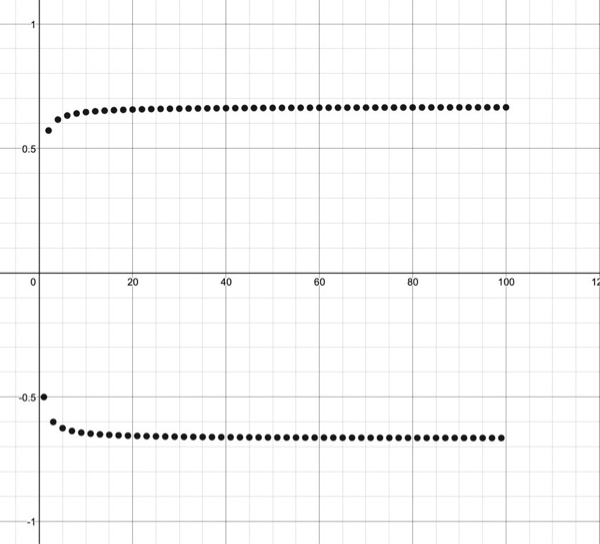
\includegraphics[width=0.5\textwidth,height=\textheight]{Image.png}

\hypertarget{example-2}{%
\subsection*{Example 2}\label{example-2}}
\addcontentsline{toc}{subsection}{Example 2}

\BeginKnitrBlock{example}
{\label{exm:ex2} }Consider the sequence \((a_n)_{n}\) defined by \[a_n = \frac{1}{n^2} - (-1)^n + 2.\] Find \(\limsup_{n \to \infty} a_n\) and \(\liminf_{n \to \infty} a_n\).
\EndKnitrBlock{example}

\textbf{Solution}
First, note that for any \(j\in\mathbb{N}\), \(a_{2j} \leq 2 \leq a_{2j-1}\). But this time, we find that both \((a_{2j})_j\) and \((a_{2j-1})_j\) are decreasing sequences! In this case, the argument used in Example \ref{exm:ex1} will only work for \(\liminf_{n\to\infty} a_n.\) Try using that argument to show that \[\liminf_{n\to\infty}a_n = 1.\] For \(\limsup_{n\to\infty} a_n\), we have to look towards the start of the sequence. To this end, fix \(k \in \mathbb{N}\). Then,
\begin{align*}
\sup_{n\geq k}a_n &= \sup_{2j-1 \geq k} a_{2j - 1} \; \; &&\text{(since only the odd elements are $\geq 2$)}\\
&=\begin{cases}
a_k \; \text{if $k$ is odd},\\
a_{k+1} \; \text{if $k$ is even}\end{cases} \; \; &&\text{(because $(a_{2j-1})_j$ is a decreasing sequence)}\\
&=\begin{cases}
\frac{1}{k^2} + 3 \; \text{if $k$ is odd},\\
\frac{1}{(k+1)^2} + 3 \; \text{if $k$ is even}\end{cases}
\end{align*}

In both cases, as \(k \to \infty\), \(\sup_{n\geq k }a_n \to 3\), so \(\limsup_{n \to \infty} a_n = 3\).

\hypertarget{example-3}{%
\subsection*{Example 3}\label{example-3}}
\addcontentsline{toc}{subsection}{Example 3}

\BeginKnitrBlock{example}
{\label{exm:ex3} }Consider the sequence \((a_n)_{n}\) defined by \[a_n = \cos\left(\frac{n\pi}{3}\right).\] Find \(\limsup_{n \to \infty} a_n\) and \(\liminf_{n \to \infty} a_n\).
\EndKnitrBlock{example}
Note that this time, you can't split \((a_n)_n\) up into two monotonic subsequences, so neither of the two methods in the previous examples work. So, we need to be crafty.

It's always handy to have an idea of what the \(\liminf\) and \(\limsup\) might be. Since \(\left\lvert\cos\left(\frac{n\pi}{3}\right)\right\rvert \leq 1\) for all \(n \in \mathbb{N}\), and \(\frac{(-1)^n}{n} \to 0\) as \(n \to \infty\), we (hopefully) would guess that \[\liminf_{n\to\infty}a_n = -1, \quad \text{and} \quad \limsup_{n \to \infty} a_n = -1.\] So how do we go about showing these?

\textbf{Solution}
Firstly, recall that the \(\limsup\) is the largest limit of any subsequence of \((a_n)_n\). Take \(n_j = 6j\), then \[a_{n_j} = \cos\left(\frac{6j\pi}{3}\right) + \frac{(-1)^{6j}}{6j} = 1 + \frac{1}{6j} \to 1, \; \text{as} \; j \to \infty.\]

So, \(\lim_{j \to \infty} a_{n_j} = 1\), hence \(\limsup_{n \to \infty} a_n \geq 1\).

To show that \(\limsup_{n \to \infty} a_n \leq 1\), recall that for sequences \((b_n)_n\) and \((c_n)_n\), \[\limsup_{n \to \infty}(b_n + c_n) \leq \limsup_{n \to \infty}b_n + \limsup_{n \to \infty}c_n.\] Taking \[b_n = \cos\left(\frac{n\pi}{3}\right), \; \text{and} \; c_n = \frac{(-1)^n}{n},\] we have that \[\limsup_{n \to \infty} b_n = 1, \; \text{and}\] \[\limsup_{n \to \infty} c_n = 0 \quad \text{(as $(c_n)_n$ converges to $0$)}.\] Hence,
\[\limsup_{n \to \infty} a_n = \limsup_{n \to \infty}(b_n + c_n) \leq 1 + 0 = 1.\]

Combining the two inequalities we have found allows us to conclude that \(\limsup_{n \to \infty} a_n = 1.\)

Have a go at proving that \(\liminf_{n \to \infty} a_n = -1\). You'll need:

\begin{itemize}
\tightlist
\item
  \(\liminf\) is the smallest limit of any subsequence of \((a_n)_n\).
\item
  \(\liminf_{n \to \infty}(b_n + c_n) \geq \liminf_{n \to \infty}b_n + \liminf_{n \to \infty}c_n.\)
\end{itemize}

\end{document}
